\section{Reinforcement Learning}\label{rl}
According to Sutton and Barto's seminal text, reinforcement learning (RL) is a branch of machine learning, based on trial-and-error, that is concerned with sequential decision making \cite{Sutton2018}. An RL agent exists in an environment. Within the environment it can act, and it can make observations of it's state and receive rewards. These two discrete steps, action and observation, are repeated indefinitely with the agent's goal being to make decisions so as to maximise its long term reward --- this scenario is represented diagramatically in Figure \ref{fig:209_reinforcement_learning_problem}.

\begin{figure}[h]
	\centering
	% Additional styles
\tikzstyle{block} = [rectangle, draw, text width=8em, text=white, text centered, rounded corners, minimum height=4em, line width=0.5mm]
    
\tikzstyle{line} = [draw, -latex]

\begin{tikzpicture}[node distance = 6em, auto, thick]
    \node [block, fill=blue!25!gray] (Agent) {\Large Agent};
    \node [block, below of=Agent, fill=green!25!gray] (Environment) {\Large Environment};
    
     \path [line] (Agent.0) --++ (4em,0em) |- node [near start]{Action} (Environment.0);
     \path [line] (Environment.190) --++ (-6em,0em) |- node [near start] {Observation} (Agent.170);
     \path [line] (Environment.170) --++ (-4.25em,0em) |- node [near start, right] {Reward} (Agent.190);
\end{tikzpicture}

	\caption[Reinforcement learning model overview]{Reinforcement learning can be thought of as two discrete steps: action and observation. The agent takes an action and receives a reward. The action causes the agent to change state in the environment.}
	\label{fig:209_reinforcement_learning_problem}
\end{figure}

One of the most common ways to represent the RL problem is to model the environment as a set of discrete probabilistic transitions between states, for a set of possible actions that can be selected by the agent. A state transition presents the agent with a reward signal that informs the agent whether an action taken was good or bad. This environmental architecture is referred to as a Markov Decision Process (MDP). It is the agent's objective to maximise the reward it will receive in the future. An agent can achieve this by learning an optimal policy which maps environment states to actions. Learning such a policy is key idea in RL, and the agent achieves this by experimentation.

%------------------------ SS: MDP

\subsection{Markov Decision Process}
Bellman's pioneering work on the Markov Decision Process (MPD) provided the necessary architecture to develop RL algorithms \cite{Bellm1957}. His work considered an agent that exists in some environment described by a set of discrete states $S$. At any discrete point in time the agent can take an action from the set of possible actions $A$. When the agent takes an action in a given state, the agent receives some reward that is assigned according to a reward function $R: S \times A \times S \to [R_{min}, R_{max}]$. Fundamental to Bellman's MDPs were the state transition dynamics which were defined by probabilities: if an agent is in a given state, $s \in S$, and takes action, $a \in A$, this will transition the agent to a new state, $s' \in S$, and yield reward, $r \in R$, with some given probability. This set of probabilities are assigned by a state transition function $P: S \times A \to S$. Generally, the a single reward is bound to a state transition so function $P$ can be thought to assign a state and reward. The function $P$, and it's simpler notation $p$, is typically written as
\begin{equation}
	P(S_{t+1} = s', \ R_{t+1} = r \ | \ S_t = s, \ A_t = a) = p(s', r \ | \ s, a). \label{eq:202}
\end{equation}

The set of parameters outlined above, and expression \ref{eq:202}, make up a framework referred to as an MDP.

\begin{figure}[h]
\centering
% Additional styles
\tikzstyle{blockn} = [rectangle, draw, text width=8em, text centered, rounded corners, minimum height=4em]
    
\tikzstyle{line} = [draw, -latex]

\tikzset{
    block/.style={
        draw,
        rectangle split,
        rectangle split parts=2,
        text centered,
        text width=8em,
        rounded corners,
        minimum height=4em
        }
}


\begin{tikzpicture}[node distance = 6em, auto, thick]
    \node [blockn, fill=blue!25!gray, text=white] (Agent) {\Large Agent};
    \node [block, below of=Agent, rectangle split empty part height=1cm, rectangle split part fill={green!20!gray,white!80!green}] (Environment) {\Large\textcolor{white}{MDP} \nodepart{second} \scriptsize $\begin{aligned}
   		s_{t+1} &\sim  P( \ \cdot \ | \ s_t,a_t )\\
   		r_{t+1} &\sim R(s_t, a_t, s_{t+1})
    \end{aligned}$};
    
     \path [line] (Agent.0) --++ (4em,0em) |- node [near start]{$a_t$} (Environment.-10);
     \path [line] (Environment.200) --++ (-6em,0em) |- node [near start] {$s_t$} (Agent.170);
     \path [line] (Environment.180) --++ (-4.25em,0em) |- node [near start, right] {$r_t$} (Agent.190);
\end{tikzpicture}

\caption[MDP model of reinforcement learning]{Reinforcement learning using an MDP architecture to model state transitions in the environment}
\label{fig:210_reinforcement_learning_problem_mdp}
\end{figure}

%------------------------ SS: Returns and Policy

\subsection{Returns, Episodes, and Policy} \label{rep}
In addition to  developing the MDP framework, Bellman was also responsible for key developments in a field of research called dynamic programming (DP) \cite{Bellm1954}. Assuming that the agent has complete knowledge of the state transition probabilities of an environment, DP algorithms can be used to determine analytical solutions for the problem of how an agent should behave to maximise it's cumulative reward \cite{Bellm1954, Howard1960}. This idea was originally thought to be distinct from RL. The main difference is that DP provides the agent with complete knowledge of it's environment, whereas RL agents have no knowledge of environment dynamics and must learn them as well as how to maximise their cumulative reward \cite{Sutton2018}. Many researchers made links between DP and RL \cite{Bellm1959, Witten1977, Werbos1987}, but it wasn't until 1989 that Watkins presented the first formal treatment of RL in an MDP framework. Watkin's work showed that DP algorithms could be modified for use with RL problems \cite{Watkins1989}. Central ideas used in DP algorithms include episodes, returns, and policies \cite{Sutton2018}.

The set of states, action, and rewards that an agent encounters before arriving at a terminal state is defined as an episode. The set of states and actions (without rewards) is often referred to as the trajectory, $\tau$. It is the agent's goal to take actions such that it maximises the sum of all the rewards as it concludes an episode. The cumulative sum of rewards is called the return. Consider an agent taking an action at each discrete time step, $t$, and receiving reward, $r_t$, after each action. If there are $N$ discrete time steps before the agent reaches a terminal state, Bellman defines the return as:
\begin{equation}
	G_t = \sum_{k = 0}^{N-1} r_{t + k}. \label{eq:203}
\end{equation}

Rewards received in the future are often perceived as less valuable than rewards received in the present. To account for this Bellman used a discount factor applied to each reward in the sequence. Letting $\gamma \in [0,1]$ then \ref{eq:203} becomes
\begin{equation}
	G_t = \sum_{k = 0}^{N-1}\gamma\mystrut^k r_{t+k}. \label{eq:204}
\end{equation}

Finally, in order for the agent to take actions it must have a belief of what action it should take, given it's current state. This belief is called a policy and denoted as $\pi$ \cite{Sutton2018}. Sutton and Barto define a  policy as the mapping of states to actions i.e. a rule that determines what actions the agent should take for a given state. A policy can be deterministic, and depend only on the state, $\pi(s)$, or stochastic, $\pi(a|s)$, such that it defines a probability distribution over the actions, for a given state. An optimal policy, denoted $\pi*$, is a policy which will maximise the return an agent receives over an episode.

%------------------------ SS: Value Function and Bellman

\subsection{Value Function and the Bellman Equations}
The basic principal of dynamic programming is to assign a value to each state that informs an agent how useful a state is to achieving a high cumulative reward. Watkins refers to the creation of systems to assign values to states as the credit assignment problem \cite{Watkins1989}. Bellman's approach to solving credit assignment was to develop mathematical functions to assign values to states \cite{Bellm1954}. Bellman's \textit{value function}, $V_{\pi}(s)$ , is defined as the expected sum of the discounted return, $G_t$, that the agent will receive while following policy $\pi$ from a particular state $s$. Mathematically, this is expressed as
\begin{equation}
	V_{\pi}(s) = \mathbb{E}_{\pi} \big( G_t \ | \ s_t = s \big) = \mathbb{E}_{\pi} \bigg( \sum_{k = 0}^{\infty} \gamma\mystrut^k r_{t+k} \ | \ s_t = s \bigg). \label{eq:205}
\end{equation}

The state value function was useful to Bellman because it provided a way to check if one policy was better than another policy. It is clear an agent would prefer policy $\pi$ over some other policy $\pi'$ if the expected return from using policy $\pi$ is greater than the expected return from using policy $\pi'$ for all $s \in S$. Since the state value function is defined by the expected return, Bellman expressed this idea in state value function terms i.e. if policy $\pi$ is preferred to $\pi'$ then $V_{\pi}(s) \geq V_{\pi'}(s)$ for all $s \in S$. The optimal policy, $\pi^*$, yields the best state value function, $V^*(s)$, referred to as the optimal state value function and defined as:
\begin{equation}
	V^*(s) = \max_{\pi} V_{\pi}(s), \ \forall \ s \in S.
\end{equation}

Although the state value function provides a way to compare one policy against another policy, it can not be used to specify the policy it evaluates. Bellman developed a variation of equation \ref{eq:205} called the \textit{state-action value function} that can evaluate and specify a policy. The state-action value function, $Q_{\pi}(s,a)$, is defined as the expected sum of the discounted return, $G_t$, that the agent will receive if it takes action $a$ in state $s$, and then follows policy $\pi$ thereafter. Mathematically, this is expressed as:
\begin{equation}
	Q_{\pi}(s, a) = \mathbb{E}_{\pi} \big( G_t \ | \ s_t = s, \ a_t = a \big) = \mathbb{E}_{\pi} \bigg( \sum_{k = 0}^{\infty} \gamma\mystrut^k r_{t+k} \ | \ s_t = s, \ a_t = a \bigg). \label{eq:206}
\end{equation}

Similarly to the state value function, the state-action value function's optimal form, $Q^*(s,a)$, can be defined as:
\begin{equation}
	Q^*(s,a) = \max_{\pi} Q_{\pi}(s,a), \ \forall \ s \in S, \ a \in A.
\end{equation}

To extract the policy $\pi$ from a state-action value function $Q_{\pi}$ the action corresponding to the largest state-action value is chosen for each given state. This is called the greedy policy and is defined, for each $s \in S$, as:
\begin{equation}
	\pi (a | s) = % 
	   \begin{cases}
	   		1 \ \ \text{if} \ \ a = \arg\max_{a'} Q(s,a') \\
	   		0 \ \ \text{if} \ \ a \neq \arg\max_{a'} Q(s,a')
	   \end{cases} \label{eq:210}
\end{equation} 

Bellman used the value functions presented in \ref{eq:205} and \ref{eq:206} to formulate recursive expressions which could then be used to solve the DP problem \cite{Bellm1957}. These are known as the \textit{Bellman equations}. Letting $A(s)$ be the set of actions available in state $s$, if the agent is operating under the optimal policy $\pi^*$ then it is true that
\begin{equation}
	V^*(s) = \max_{a \in A(s)} Q_{\pi*}(s,a). \label{eq:207}
\end{equation}

Using the notation shown in equation \ref{eq:202}, equation \ref{eq:207} can be rewritten using equation \ref{eq:206}
\begin{equation}
	V^*(s) = \max_{a} \sum_{s',r} p(s', r \ | \ s, a)[r + \gamma V^*(s')]. \label{eq:208}
\end{equation}  

Equation \ref{eq:208} is referred to as the Bellman optimality equation for $V^*(s)$. The Bellman optimality equation for $Q^*(s,a)$ is
\begin{equation}
	Q^*(s,a) = \sum_{s'} p(s', r \ | \ s, a)[r + \gamma \max_{a'} Q^*(s',a')]. \label{eq:209}
\end{equation}

If the transition probabilities and rewards are known to the agent then the Bellman opitmality equations can be solved iteratively, which is known as dynamic programming \cite{Bellm1957}. Algorithms which assume known transition probabilities and rewards are collectively referred to as \textit{model-based} algorithms. Most RL problems assume state transition probabilities are unknown. The collection of algorithms that provide solutions to these problems are called \textit{model-free} algorithms.

%------------------------ SS: Value Function Based Methods

\subsection{Value Function Based Methods}
Model free methods can be applied to any RL problem since they do not require a model of the environment. Algorithms that try to solve the RL problem by estimating the optimal state-action value function, $Q^*$, and inferring the optimal policy from it are referred to as value function based methods. Figure \ref{fig:211_families_of_RL_algorithms} provides a high level overview of value function based methods. The most common value function based methods are Monte Carlo and temporal difference approaches.

\begin{figure}[h]
	\centering
	\resizebox{\textwidth}{!}{% Additional styles
\tikzstyle{blockn} = [rectangle, draw, text width=4em, text centered, rounded corners, minimum height=4em]
    
\tikzstyle{line} = [draw, -latex]

\tikzset{
    block/.style={
        draw,
        rectangle split,
        rectangle split parts=2,
        text centered,
        text width=8em,
        rounded corners,
        minimum height=4em
        }
}


\begin{tikzpicture}[node distance = 6em, auto, thick]
    
	% Environment node
	\node [block, rectangle split empty part height=1cm, rectangle split part fill={green!20!gray,white!80!green}] (Environment) {\Large\textcolor{white}{Experience} \nodepart{second} \scriptsize $\begin{matrix}
	  		s_0 	& r_0 	  	& a_0  \\
	  		s_1 	& r_1 	  	& a_1  \\
	  				& \vdots	&	   \\
	  		s_{t-1} & r_{t-1} 	& a_{t-1}
	\end{matrix}$};
	
	\node [coordinate, right of=Environment, node distance=7cm] (c1) {};
	
	\node [blockn, above of=c1, fill=blue!25!gray, text=white, opacity=0.5] (dynamic) {\Large $P$, $R$};
	
	\node [blockn, right of=c1, node distance=4cm, fill=blue!25!gray, text=white] (value) {\Large $Q$};
	
	\node [coordinate, right of=value, node distance=4cm] (c2) {};
	
	\node [blockn, below of=c2, node distance=2.5cm, fill=blue!25!gray, text=white] (policy) {\Large $\pi$};
	
	\path [line, color=gray] (Environment.0) --++ (4em,0em) |- node [near end]{\small dynamic prog.} (dynamic.180);
	
	\path [line, color=gray] (c1) |- node [near end] {\small policy based} (policy);
	
	\path [line] (Environment.-20) --++ (4em,0em) -| node [near start] {\small model free} (c1) -- node {\small value func. based} (value.180);
	
	\path [line, color=gray] (dynamic.0) -| (value.90);
	\path [line, color=gray] (dynamic.0) -| (policy.90);
	\path [line] (value.0) -| (policy.90);
	
\end{tikzpicture}}
	\caption[RL approaches: Value Based]{Value based approaches try to estimate the state-action value function}
	\label{fig:211_families_of_RL_algorithms}
\end{figure}

%------------------------ SSS: Monte Carlo Methods

\subsubsection{Monte Carlo Methods}
Sutton and Barto were the first to introduce a version of the Monte Carlo (MC) control algorithm for estimating state-action value functions \cite{Sutton2018}. The MC control algorithm is based on an iterative approach that takes a sample of episodic sequences consisting of states, actions, and rewards. Sequences are obtained from the agent interacting with the environment, using some policy $\pi$. This is called the \textit{policy evaluation} step. Once an episode is completed, the state-action value function, $Q_{\pi}(s,a)$, is updated for each discrete state-action pair visited. This second step is called the \textit{policy improvement} step.

\begin{figure}[h]
	\centering
	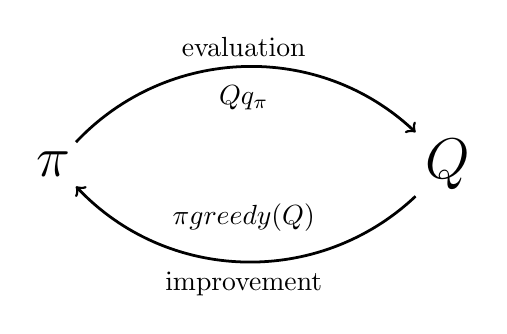
\begin{tikzpicture}
	
	% Create nodes
	\node (A) {\huge$\pi$};
	\node[right of=A, node distance=5cm] (B) {\huge$Q$};
	
	% Create arrow
	\draw[->, line width=1pt] (A) edge[bend left=45] node[below=0.1cm] {$Q \rightsquigarrow q_\pi $} node[above] {evaluation} (B);
	
	% Create arrow
	\draw[->, line width=1pt] (B) edge[bend left=45] node[below] {improvement} node[above=0.25cm] {$\pi \rightsquigarrow greedy(Q)$} (A);
	
\end{tikzpicture}
	\caption[Monte Carlo iterative approach]{The Monte Carlo algorithm takes a policy evaluation step and policy improvement step, for each episodic iteration.}
	\label{fig:210_monte_carlo_methods}
\end{figure}

Sutton and Barto found that during the policy evaluation step, if the agent was allowed to select the action with a greedy policy (\ref{eq:210}) from the current iteration of the state-action value function, then MC control would not always converge to the optimal state-action value function. The problem with using the greedy policy is that it can cause the agent to over commit to locally promising but globally poor solutions. This is due to the agent not sufficiently exploring the state-action value space, and is especially problematic during the early stages of the algorithm where the agent has little knowledge about the environment.

The most common method of overcoming this problem is to use an $\epsilon$-greedy policy instead of the greedy policy. The basic idea behind the $\epsilon$-greedy policy is to select the greedy action most of the time, and select non-greedy actions the other times. This is achieved by setting a parameter, $\epsilon \in [0,1]$, which allows the agent to select non-greedy actions with a non-zero probability. The $\epsilon$-greedy policy is defined as:
\begin{equation}
   \pi (a | s) = % 
   \begin{cases}
   		1 - \epsilon \ \ \text{if} \ \ a = \arg\max_{a'} Q(s,a') \\
   		\frac{\epsilon}{|A|-1} \ \ \text{if} \ \ a \neq \arg\max_{a'} Q(s,a')
   \end{cases} \label{eq:211}
\end{equation}

Originally, for a given state-action pair, $(s,a)$, the policy improvement step updated the state-action value function, $Q(s,a)$, using an average approach. The average value used for the update was derived from the returns of all visits, past and present, to a given state-action value pair. This approach worked; however, learning in the later stages of the algorithm was reduced because the averaging algorithm placed a uniform importance on all stages of learning. To overcome this problem, Sutton and Barto employed a coarser update rule using the difference between observed returns and the current state-action value function. The update value was then multiplied by some value $\alpha \in [0,1]$ to ensure that the update steps were not too large. If update steps are too large, this may prevent the algorithm convergence to $Q^*$. For some point in time $t$, if $S_t$ is the state, $A_t$ is the action, and $G_t$ is the observed return for completion of the current episode, then update rule can be written as:
\begin{equation}
	Q(S_t, A_t) \gets Q(S_t, A_t) + \alpha[G_t - Q(S_t, A_t)] \label{eq:212}
\end{equation}

The MC implementation using the $\epsilon$-greedy policy \ref{eq:211} for the evaluation step, and the constant $\alpha$ update rule in \ref{eq:212} is referred to as the Constant $\alpha$ Monte Carlo control algorithm. The algorithm is shown in listing \ref{alg:01}. Note that the algorithm returns as approximation of the optimal state-action value function, and the optimal policy can be extracted using the greedy policy in \ref{eq:210}.

\begin{algorithm}[h]
	\caption{Constant $\alpha$ Monte Carlo Control}
	\label{alg:01_monte_carlo}
	\begin{algorithmic}[1]
		\State{\textbf{Input:} $\mathtt{num\_episodes}$, $\alpha$, $\epsilon_i$}
		\State{\textbf{Output:} $Q$ ($\approx Q^*$ if $\mathtt{num\_episodes}$ is large enough)}
		\State{Initialise $Q$ such that $Q(s,a) = 0 \ \text{for all} \ s \in A \ \text{and} \ a \in A$}
		\For{$i \gets 1:\mathtt{num\_episodes}$}
			\State{$\epsilon \gets \epsilon_i$}
			\State{$\pi \gets \epsilon-\text{greedy}$}
			\State{Generate and episode $S_0, A_0, R_1,\dots,S_T$ using $\pi$}
			\For{$t \gets 0:(T-1)$}
				\If{$(S_t, A_t)$ is a first visit}
					\State{$Q(S_t, A_t) \gets Q(S_t, A_t) + \alpha(G_t - Q(S_t, A_t))$}
				\EndIf
			\EndFor
		\EndFor
		\State{\textbf{return} $Q$}
	\end{algorithmic} \label{alg:01}
\end{algorithm}

%------------------------ SSS: Temporal Difference Methods

\subsubsection{Temporal Difference Methods}
Monte Carlo (MC) methods collect experience from an episode, and update the policy once the episode is complete. This approach works for environments that have short episodes, but becomes computationally intractable for environments where an episode takes a long time to reach a terminal state, or for continuing tasks that never reach a terminal state. Temporal difference (TD) methods address this problem.

TD methods take an almost identical approach to MC methods, except they perform state-action value function updates after every time step during an episode instead of waiting until episode completion. This is achieved by estimating the return for a given time step, since it would be unknown during an episode. More concretely, for a given state-action pair, $(S_t, A_t)$, which transitions the environment to state $S_{t+1}$, the return is estimated using the transition reward, $R_{t+1}$, and the state-action value function estimate for the subsequent state, assuming a greedy policy:
\begin{equation}
	G_t \approx R_{t+1} + \max_{a}Q(S_{t+1}, a) \label{eq:213}
\end{equation}

Along with his highly influential integration of RL with MDPs and DP, Watkins developed one of the most widely used TD algorithms called Q-learning \cite{Watkins1989}. Watkins used \ref{eq:213} to modify the update rule \ref{eq:213} as follows:
\begin{equation}
	Q(S_t, A_t) \gets Q(S_t, A_t) + \alpha[R_{t+1} + \gamma \max_{a} Q(S_{t+1},a) - Q(S_t, A_t)] \label{eq:214}
\end{equation}

The Q-learning algorithm is summarised in listing \ref{alg:02}.

\begin{algorithm}[h]
	\caption{Q-learning}
	\label{alg:02_q_learning}
	\begin{algorithmic}[1]
		\State{\textbf{Input:} $\mathtt{num\_episodes}$, $\alpha$, $\epsilon_i$}
		\State{\textbf{Output:} value function $Q$ ($\approx Q^*$ if $\mathtt{num\_episodes}$ is large enough)}
		\State{Initialise $Q$ such that $Q(s,a) = 0 \ \text{for all} \ s \in S \ \text{and} \ a \in A$}
		\For{$i \gets 1:\mathtt{num\_episodes}$}
			\State{$\epsilon \gets \epsilon_i$}
			\State{Observe initial state $S_0$}
			\State{$t \gets 0$}
			\Repeat
				\State{Select an action $A_t$ using policy derived from $Q$ (e.g. $\epsilon$-greedy)}
				\State{Carry out action $A_t$}
				\State{Observe reward $R_{t+1}$ and new state $S_{t+1}$}
				\State {$Q(S_t,A_t) \gets Q(S_t,A_t) + \alpha[R_{t+1} + \gamma\max_{a} Q(S_{t+1},a) - Q(S_t,A_t)]$}
				\State{$t \gets t+1$}
			\Until{$S_t$ is terminal}
		\EndFor
		\State{\textbf{return} Q}
	\end{algorithmic} \label{alg:02}
\end{algorithm}

%------------------------ SS: Policy Search Methods

\subsection{Policy Search Methods}
Policy search methods are another class of RL algorithms that do not use value functions to determine state to action policy mappings. Figure \ref{fig:2xx_families_of_RL_algorithms} provides a high level overview of policy search methods compared to dynamic programming and value function based methods.

\begin{figure}[h]
	\centering
	\resizebox{\textwidth}{!}{% Additional styles
\tikzstyle{blockn} = [rectangle, draw, text width=4em, text centered, rounded corners, minimum height=4em]
    
\tikzstyle{line} = [draw, -latex]

\tikzset{
    block/.style={
        draw,
        rectangle split,
        rectangle split parts=2,
        text centered,
        text width=8em,
        rounded corners,
        minimum height=4em
        }
}


\begin{tikzpicture}[node distance = 6em, auto, thick]
    
	% Environment node
	\node [block, rectangle split empty part height=1cm, rectangle split part fill={green!20!gray,white!80!green}] (Environment) {\Large\textcolor{white}{Experience} \nodepart{second} \scriptsize $\begin{matrix}
	  		s_0 	& r_0 	  	& a_0  \\
	  		s_1 	& r_1 	  	& a_1  \\
	  				& \vdots	&	   \\
	  		s_{t-1} & r_{t-1} 	& a_{t-1}
	\end{matrix}$};
	
	\node [coordinate, right of=Environment, node distance=7cm] (c1) {};
	
	\node [coordinate, below of=c1, node distance=0.67cm] (test1) {};
	
	\node [blockn, above of=c1, fill=blue!25!gray, text=white, opacity=0.5] (dynamic) {\Large $P$, $R$};
	
	\node [blockn, right of=c1, node distance=4cm, fill=blue!25!gray, text=white, opacity=0.5] (value) {\Large $Q$};
	
	\node [coordinate, right of=value, node distance=4cm] (c2) {};
	
	\node [blockn, below of=c2, node distance=2.5cm, fill=blue!25!gray, text=white] (policy) {\Large $\pi$};
	
	\path [line, color=gray] (Environment.0) --++ (4em,0em) |- node [near end]{\small dynamic prog.} (dynamic.180);
	
	\path [line, color=gray] (test1) -- (c1) -- node {\small value func. based} (value.180);
	
	\draw (Environment.-20) --++ (4em,0em) -| node [near start] {\small model free} (test1);
	
	\path [line] (test1) |- node [near end] {\small policy based} (policy);
	
	\path [line, color=gray] (dynamic.0) -| (value.90);
	\path [line, color=gray] (value.0) -| (policy.90);
	\path [line, color=gray] (dynamic.0) -| (policy.90);
	
\end{tikzpicture}}
	\caption[RL approaches: Policy search]{Policy search approaches try to estimate the policy directly without using state-action values.}
	\label{fig:2xx_families_of_RL_algorithms}
\end{figure}

Instead of value functions, policy search methods use parameterised policies, $\pi(a | s;\theta)$. Parameters are represented as a vector, $\theta \in \Theta$, and changing individual elements of vector $\mathbf{\theta}$ changes how the policy maps states to actions. The novelty of this approach is that the policy is expressed as a parameterised functional form, where the function can be anything from a linear model to a neural network, although not all functions perform equally.

The basic idea behind policy search is that the agent searches directly for the optimal policy in vector space, $\Theta$. To express this idea more formally, let $J(\theta)$ denote the expected value of the discounted return of trajectory $\tau$, for policy $\pi(a|s;\theta)$. Mathematically, this is written as:
\begin{equation}
	J(\theta) = \mathbb{E}_{\tau \sim \pi(a|s;\theta)} \bigg( \sum_{t=1}^{\infty} \gamma\mystrut^{t-1} r_t \bigg). \label{eq:215}
\end{equation}

Finding the optimal policy, for policy search, can now be expressed as a maximisation problem of $J(\theta)$, that is: 
\begin{equation}
	\pi^* = \pi\big(a|s;\arg\max_{\theta} J(\theta)\big) \label{eq:216}
\end{equation}

Expressing the policy search problem this way allows for the application of many different optimisation algorithms. One simple approach is to use a hill climbing algorithm. Suppose the agent possess some policy, $\pi_{\theta}$, which it can roll-out in the environment and get some return, $G$. It can then slightly modify $\theta$ to get some marginally different policy, say $\pi_{\theta'}$. The agent could then roll-out the new policy in the environment and receive a return $G'$. If $G' > G$, then hill climbing would discard policy $\pi_{\theta}$ in favour of $\pi_{\theta'}$; and if $G' < G$, then hill climbing retains policy $\pi_{\theta}$. Continued iterations of the above would see the agent's policy converge to an optimal policy, although this is not guaranteed to be globally optimal.

Another well known algorithm that is used to solve \ref{eq:216} is gradient ascent. In gradient ascent, the parameter update direction is given by the gradient $\nabla_{\theta} J(\theta)$ as it points in the direction of steepest ascent of the expected return. Provided $\nabla_{\theta} J(\theta)$ exists, the parameter update rule is expressed as:
\begin{equation}
	\theta \gets \theta + \alpha \nabla_{\theta}J(\theta),
\end{equation}
where $\alpha$ is a user-specified learning rate.

Policy search has better convergence properties and can learn stochastic policies which are not possible with value based approaches

NEED TO CONCLUDE THIS SECTION